\documentclass[12pt, openany, letterpaper]{memoir}
\usepackage{NotesStyle}

\begin{document}
\title{CHEM 3610 Lecture Notes\\--On Projections--}
\author{Matthew Rowley}
\date{Fall 2016}
\mainmatter
\maketitle
\section*{Projection onto a Polynomial Basis}

Remember that any function can be represented as a sum of all the functions in a basis set, but each basis set function must be \emph{scaled} by a co-efficient:

\begin{equation*}
	\Psi = \sum_i{c_i \phi_i}
\end{equation*}

Our goal is to find the values of $c_i$ so that we can know how much each basis function $\phi_i$ contributes to the function $\Psi$. This can also be interpreted as a measure of how \emph{similar} is each basis function to $\Psi$.

\vspace{1em}
This can be accomplished with the simple integral, which can be called the \emph{overlap} integral:
\begin{equation*}
	c_i = \braket{\phi_i}{\Psi} = \int{\phi_i^*\Psi d\tau}
\end{equation*}

\vspace{1em}
Consider the following basis set. These are now normalized, unlike those I showed you in class. Note that these are orthonormal only over the interval $[-1,1]$. 
\begin{equation*}
	\phi_0(x) = \frac{1}{\sqrt{2}}, ~~ \phi_1(x) = \sqrt{\frac{3}{2}}x, ~~ \phi_2(x) = \frac{\sqrt{15}}{4}\left(x^2-\frac{1}{3}\right), ~~ \phi_3(x) = \sqrt{\frac{175}{8}}\left(x^3 -\frac{3}{5}x\right)
\end{equation*}

and the function:
\begin{equation*}
	F(x) = \sin{x}+\frac{1}{2}
\end{equation*}

Projecting onto each basis function in turn gives:
\begin{equation*}
	c_0 = \int_{-1}^{1}\frac{1}{\sqrt{2}}\left(\sin{x}+\frac{1}{2}\right)dx = \frac{1}{\sqrt{2}}\left[-\cos{x}+\frac{1}{2}x\right]_{-1}^{1} = \frac{1}{\sqrt{2}}
\end{equation*}

\begin{equation*}
	c_1 = \int_{-1}^{1}\sqrt{\frac{3}{2}}x\left(\sin{x}+\frac{1}{2}\right)dx = \sqrt{\frac{3}{2}}\left[\sin{x} -x\cos{x} +\frac{1}{4}x^2\right]_{-1}^{1} =  \sqrt{6}\left(\sin(1)-\cos(1)\right)
\end{equation*}

\begin{equation*}
	c_2 = \int_{-1}^{1}\frac{\sqrt{15}}{4}\left(x^2-\frac{1}{3}\right)\left(\sin{x}+\frac{1}{2}\right)dx = 0 ~(exactly)
\end{equation*}

\begin{equation*}
	c_3 = \int_{-1}^{1}\sqrt{\frac{175}{8}}\left(x^3-\frac{3}{5}x\right)\left(\sin{x}+\frac{1}{2}\right)dx = \sqrt{14}\left(14\cos(1)-9\sin(1)\right)
\end{equation*}

The last two I did using Wolfram Alpha because the integrals do get pretty dicey. Below is a figure showing the results (the coefficients are approximate, since I found them numerically).

\begin{figure}[h!]
  \centering
  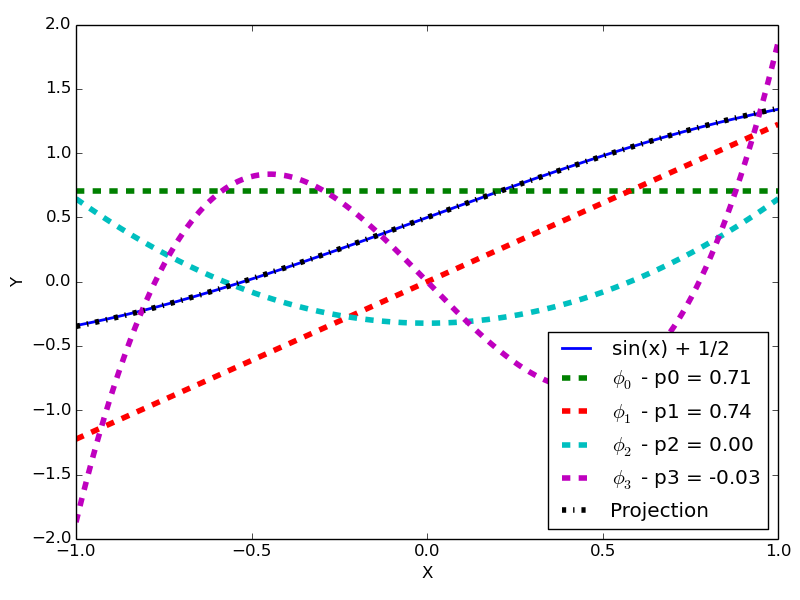
\includegraphics[width=0.93\textwidth]{figures/Projection}
\end{figure}

\section*{Projection onto a Fourier Series}

Problem P2.32 asks to project the function:
\begin{equation*}
	f(y) = y^2
\end{equation*}
onto a Fourier series basis set. In other words, find the coefficients for the following equation:
\begin{equation*}
	f(y) = d_0 + \sum_{n=1}^\infty c_n\sin\left(\frac{n\pi y}{a}\right) + d_n\cos\left(\frac{n\pi y}{a}\right)
\end{equation*}

We see that this Fourier series is a basis set consisting of three types of functions: $d_0\dfrac{1}{\sqrt{2a}}$, $c_n\dfrac{1}{\sqrt{a}}\sin\left(\dfrac{n\pi y}{a}\right)$, and $d_n\dfrac{1}{\sqrt{a}}\cos\left(\dfrac{n\pi y}{a}\right)$. Here I have strayed a bit from the derivation in class by normalizing these basis functions up front.

Now we can find the coefficients by doing the same overlap integral as before, namely:
\begin{equation*}
	c_i = \braket{\phi_i}{\Psi} = \int{\phi_i^*\Psi d\tau}
\end{equation*}

Now, we can use symmetry to simplify a few of these. We know that $f(x)=y^2$ is a function with \emph{even} symmetry, while $\sin\left(\dfrac{n\pi y}{a}\right)$ has \emph{odd} (or \emph{antisymmetric}) symmetry. The overlap integral of a product of an even and an odd function will always be 0. We would say that they are orthogonal by symmetry.  So, we know that all coefficients $c_n$ are 0.

To get the others, we must perform the integration:

\begin{equation*}
	d_0=\int_{-a}^{a}\dfrac{1}{\sqrt{2a}}y^2dy=\dfrac{1}{\sqrt{2a}}\left[\frac{1}{3}y^3\right]_{-a}^{a} = \frac{2\sqrt{2}}{6}a^{\nicefrac{5}{2}}
\end{equation*}

\begin{equation*}
\begin{array}{rcl}
	d_{n>0} &=& \dfrac{1}{\sqrt{a}}\int_{-a}^{a}y^2\cos\left(\dfrac{n\pi y}{a}\right)dy\\ \\
	
	&=&\dfrac{1}{\sqrt{a}}\left[\left(\dfrac{a}{n\pi}\right)^3\left(\left(\dfrac{n\pi}{a}\right)^2y^2-2\right)\sin{\left(\dfrac{n\pi y}{a}\right)}+\left(\dfrac{a}{n\pi}\right)^3 2y \cos{\left(\dfrac{n\pi y}{a}\right)}\right]_{-a}^{a}\\ \\
	
	&=&\dfrac{1}{\sqrt{a}}\left[\dfrac{a}{n\pi}y^2\sin{\left(\dfrac{n\pi y}{a}\right)} - \left(\dfrac{a}{n\pi}\right)^3 2\sin{\left(\dfrac{n\pi y}{a}\right)}+\left(\dfrac{a}{n\pi}\right)^2 2y \cos{\left(\dfrac{n\pi y}{a}\right)}\right]_{-a}^{a}
\end{array}
\end{equation*}

Here I made a small mistake in class, so ignore your notes and instead follow what I do now. If your functions are symmetric (or antisymmetric) over your interval, then you can simplify some integrals. An odd function will integrate to zero, because any positive area will perfectly match a negative area on the other side. Consider finding the area under $f(x) = \sin(x)$ over the interval of $[-\pi,\pi]$ --- it will be zero for this reason.

Similarly, an even function will evaluate to zero over the interval because you end up subtracting a value from itself. Here consider evaluating $f(x) = \cos(x)$ over the interval of $[-\pi,\pi]$. You would get $-1 - (-1) = 0$

Remember also the rule: odd x odd = even, even x even = even. and odd x even = odd. This applies to the symmetry of functions as well as to the parity of numbers.

Unfortunately, all of the functions we are evaluating here are odd, so there is no simplification to be done except by evaluating over the interval. Fortunately, $\sin\left(\dfrac{n\pi y}{a}\right)$ still \emph{does} go to zero over the interval $[-a,a]$, just not for reasons of symmetry.

\begin{equation*}
\begin{array}{rcl}
	d_{n>0}	&=&\dfrac{1}{a}\left[\dfrac{a}{n\pi}y^2\sin{\left(\dfrac{n\pi y}{a}\right)} - \left(\dfrac{a}{n\pi}\right)^3 2\sin{\left(\dfrac{n\pi y}{a}\right)}+\left(\dfrac{a}{n\pi}\right)^2 2y \cos{\left(\dfrac{n\pi y}{a}\right)}\right]_{-a}^{a}\\ \\
	& = & \dfrac{1}{a}\left[\left(\dfrac{a}{n\pi}\right)^2 2y \cos{\left(\dfrac{n\pi y}{a}\right)}\right]_{-a}^{a}\\ \\
	
	& = & \dfrac{1}{\sqrt{a}}\left[\dfrac{2a^3}{n^2\pi^2}(-1) - \dfrac{-2a^3}{n^2\pi^2}(-1)\right] = - \dfrac{4a^{\nicefrac{5}{2}}}{n^2\pi^2} ~~ for ~~ odd ~~n\\ \\
	& = & \dfrac{1}{\sqrt{a}}\left[\dfrac{2a^3}{n^2\pi^2}(1) - \dfrac{-2a^3}{n^2\pi^2}(1)\right] = \dfrac{4a^{\nicefrac{5}{2}}}{n^2\pi^2} ~~ for ~~ even ~~n\\ \\
	& = & (-1)^n\dfrac{4a^{\nicefrac{5}{2}}}{n^2\pi^2}
\end{array}
\end{equation*}


But wait, a negative coefficient\ldots is that even a thing? Yes, it is very much a thing. Consider the curvature of cosine functions compared to the curvature of $y^2$. Cosines curve downward while $y^2$ curves upward, so we have to use the negatives of the cosine functions.

Finally, below is a plot showing how this works, for the case where $a=\pi$. 

\begin{figure}[]
  \centering
  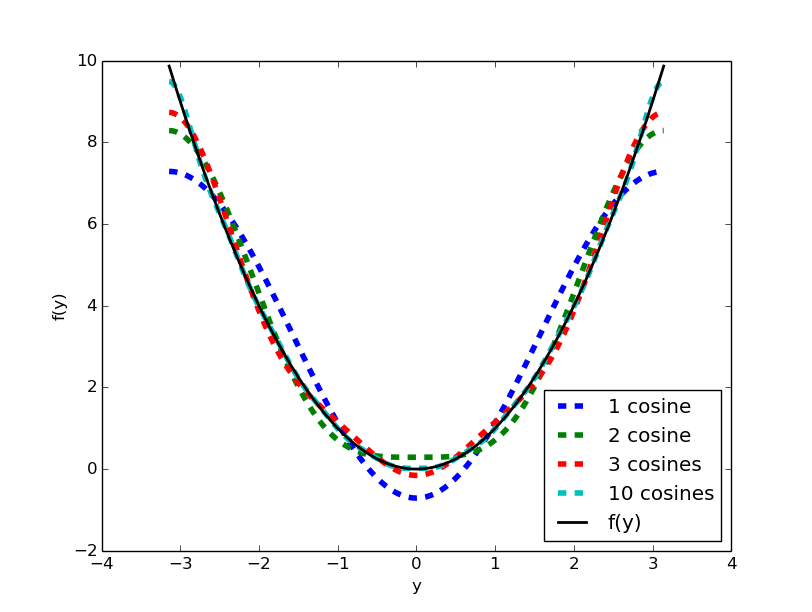
\includegraphics[width=0.93\textwidth]{figures/Fourier}
\end{figure}

\newpage
~
\newpage
\section*{Exam 1 Study Guide}

Here is a brief overview of what you need to know for this exam:

\begin{itemize}
	\item Early quantum experiments, such as:
	\begin{itemize}
		\item The spectrum of blackbody radiation
		\item The photoelectric effect
		\item Hydrogen atom emission lines
		\item Single photon diffraction
		\item Matter wave diffraction
	\end{itemize}
	\item DeBroglie Wavelengths
	\item Diffraction fringe spacing for given parameters
	\item Energy level occupancy and the Boltzmann distribution
	\item Dealing with complex numbers
	\item Spherical and Cartesian coordinate systems
	\item Operators in linear algebra
	\item Eigenfunctions and Eigenvalues
	\item Normalization of a function
	\item Orthogonality of functions
	\item Projection onto a basis set
\end{itemize}
On the following pages are the equations and formulas which will be provided to you for use during the exam.

\include{equations1}

\end{document}